\documentclass{article}
\usepackage{amsmath}
\usepackage{amssymb}
\usepackage{graphicx}
\usepackage{hyperref}
\usepackage[version=4]{mhchem}


\begin{document}
\section*{Problem}
In \(\triangle A B C, A E\) is the diameter of the circumcircle. \(A D\) is the altitude on \(B C\). Show that \(A B \times A C=A D \times A E\).\\
\centering
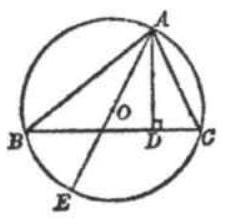
\includegraphics[width=\textwidth]{images/169(1).jpg}

\section*{Solution}
Method 1:\\
Connect \(B E\). Triangle \(A B E\) is a right triangle.\\
Since \(\angle A C B\) and \(\angle A E B\) face the same arc, \(\angle A C B=\angle A E B\).\\
We also know that \(\angle A B E=\angle A D C=90^{\circ}\).\\
Therefore \(\triangle A C D\) and \(\triangle A B E\) are similar.\\
\centering
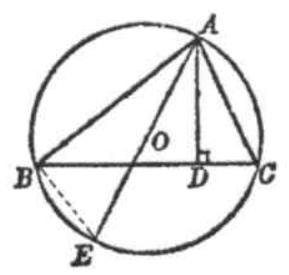
\includegraphics[width=\textwidth]{images/172(1).jpg}\\
\(\frac{A B}{A E}=\frac{A D}{A C} \quad \Rightarrow \quad A B \times A C=A D \times A E\).\\
Method 2:


Connect \(E C\). Triangle \(A E C\) is a right triangle.\\
Since \(\angle A B C\) and \(\angle A E C\) face the same arc, \(\angle A B C=\angle A E C\).\\
We also know that \(\angle A D B=\angle A C E=90^{\circ}\). Therefore \(\triangle A E C\) and \(\triangle A B D\) are similar.\\
\(\frac{A B}{A D}=\frac{A E}{A C} \quad \Rightarrow \quad A B \times A C=A D \times A E\).\\
\centering
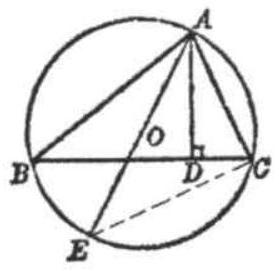
\includegraphics[width=\textwidth]{images/173.jpg}

\end{document}
